\documentclass[a4paper, 12pt]{article}
\usepackage{blindtext}
\usepackage[margin=2 cm]{geometry}
\usepackage[spanish]{babel}
\usepackage[utf8]{inputenc}
\usepackage{array}
\usepackage{amsmath}
\usepackage{graphicx}
\usepackage{ifthen}
\usepackage{commath}
\usepackage{esint}
\usepackage{mathtools}
\usepackage{listing}
\usepackage{multirow}
\usepackage{tabto}
\usepackage[backend=biber]{biblatex}
\usepackage{csquotes}
\usepackage{float}
\usepackage{amssymb}
\usepackage{physics}
\usepackage{hyperref}
\usepackage[shortlabels]{enumitem}
\selectlanguage{spanish}
\decimalpoint

\begin{document}
    \begin{center}
        \begin{Large}

            \begin{figure}[H]	
                \centering
                
\includegraphics[width = 6cm]{./img/logo_UADY.png}
                \label{uady}
            \end{figure}
            \textsc{FACULTAD DE INGENIERÍA}
                
            \medskip

            Curso Agosto - Diciembre 2021

            \medskip

            \textsc{Física Computacional}

            \medskip

            \textsl{Actividad de Aprendizaje 4}

            \medskip

            Br. Alejandro Santoscoy Rivero

            \medskip

            Dr. Francisco Ramón Peñuñuri Anguiano

            \rule{0.3\paperwidth}{0.5pt}

            \medskip

            9 de Diciembre de 2021

        \end{Large}
    \end{center}
    \pagenumbering{roman}
    \newpage
    \pagenumbering{arabic}

    \section{Problemas}

    \subsection{Problema 1}

    1. Grafique $y(x)$ para las siguientes ecuaciones diferenciales

    \begin{enumerate}[a)]
        \item $y''(x) + \sin (xy'y)+2x = 5; y(0) = 1, y'(0) = 2$ para $x \in [0,3]$
        \item $y^{(4)}+\sin xy^{(3)} + \exp (-x) y'' + y' - xy = 0$ con el vector de condiciones iniciales $Y_0 = [1,2,3,4]$, para $x \in [1,2]$ (Observe que $X_0 = 1$)
    \end{enumerate}

    Estos ejerciciso se resuelven con el método de Runge Kuta de 4to orden.

    Lo primero que se hace es definir la función en general en Octave.

    \begin{verbatim}
        function local = RK4(fun_rhs,a,b,init_cond,n_ints)
  
        nrow = n_ints+1;
        ncol = size(init_cond)(2);
        
        local = zeros(nrow,ncol);
        
        h = (b - a)/n_ints;
        
        x = zeros(nrow,1);
        y = zeros(nrow,ncol);
        x(1) = a;
        y(1,:) = init_cond;
        
        for ii=1:n_ints
            K1 = h*fun_rhs(x(ii),y(ii,:));
            K2 = h*fun_rhs(x(ii)+0.5*h, y(ii,:)+0.5*K1);
            K3 = h*fun_rhs(x(ii)+0.5*h, y(ii,:)+0.5*K2);
            K4 = h*fun_rhs(x(ii)+h, y(ii,:)+K3);
            
            x(ii+1) = x(ii) + h;
            y(ii+1,:) = y(ii,:) + (1/6)*(K1 + 2*K2 + 2*K3 + K4);
        end
        
        local = cat(2, x, y);
        end
    \end{verbatim}

    Una vez definida la función ahora es resolver cada ecuación diferencial para obtener las funciones derivadas de ellas.

    \begin{enumerate}[a)]
        \item Se está tratando de una ecuación diferencial de 2do orden, así que tenemos 2 condiciones de frontera.
        
        Primero se realiza un cambio de variable dependiente:

        \begin{align*}
            u_1 &= y \\
            u_2 &= y'
        \end{align*}

        Entonces la ecuación diferencial de puede reescribir como

        \[
            u_2'+ \sin (x u_1 u_2) + 2x = 5
        \]

        Despejando $u_2'$

        \[
            u_2' = 5 - 2x - \sin (x u_1 u_2)
        \]

        Y por reglas de igualdad, podemos decir que $u_1' = u_2$

        Teniendo estas dos funciones derivadas y las condiciones de frontera, entonces ya se puede codificar el comportamiento como

        \begin{verbatim}
            fr = @(x,y) [y(2), 5-2*x-sin(x*y(1)*y(2))]

            a=0;
            b=2;
            y0=[1,2];
            npts = 500;
            sol = RK4(fr,a,b,y0,npts);


            hold on;
            scatter(sol(:,1),sol(:,2),3,'filled');
        \end{verbatim}

        El resultado de los puntos obtenidos es la siguiente:

        \begin{figure}[ht!]
            \centering
            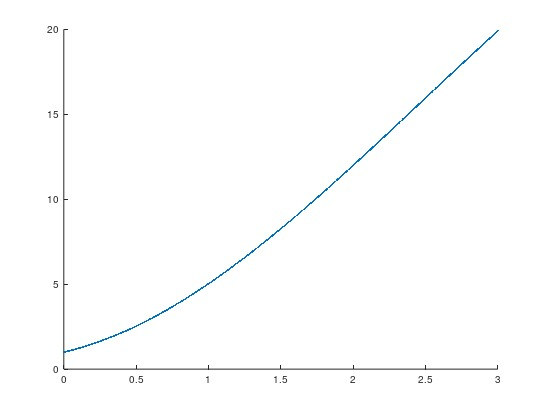
\includegraphics[width=16cm]{img/e1a.jpeg}
        \end{figure}

        \item Para la siguiente ecuación, la cual es de 4to orden, se realiza un procedimiento similar
        
        \begin{align*}
            u_1 &= y \\
            u_2 &= y' \\
            u_3 &= y'' \\
            u_4 &= y''' \\
        \end{align*}

        Entonces la ecuación se puede reescribir como

        \[
            u_4' = xu_1 - u_2 - \exp(-x)u_3 - \sin(xu_4)
        \]

        Con

        \begin{align}
            u_1' &= u_2 \\
            u_2' &= u_3 \\
            u_3' &= u_4 \\
        \end{align}

        Al escribir las funciones derivadas y las condiciones iniciales:

        \begin{verbatim}
            fr = @(x,y) [y(2),y(3),y(4),x*y(1)-y(2)-exp(-x)*y(3)
            -sin(x*y(4))]

            a=0;
            b=2;
            y0=[1,2,3,4];
            npts = 500;
            sol = RK4(fr,a,b,y0,npts);

            hold on;
            scatter(sol(:,1),sol(:,2),3,'filled');
        \end{verbatim}

        Y la gráfica queda de la siguiente manera

        \begin{figure}[ht!]
            \centering
            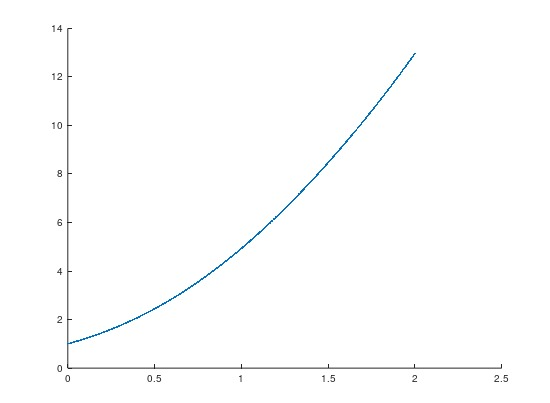
\includegraphics[width=16cm]{img/e1b.jpeg}
        \end{figure}

    \end{enumerate}

    \subsection{Problema 2}

    2. La ecuación de movimiento para un péndulo amoritugado es:

    \[
        \ddot{\theta} + \frac{c}{m} \dot{\theta} + \frac{g}{l} \sin \theta = 0  
    \]

    Tomando $m=1 kg$, $l=1m$, $g=9.8m/s^2$ y $c=0.5 Ns/m$ 7 las condiciones iniciales son $\theta(0) = \pi/2 y \dot{\theta}(0) = 0$. Haga una gráfica de la tensión en la cuerda como función del tiempo.

    Se realiza una sustitución de variables

    \[
        \omega = \dot{\theta}
    \]

    Reesbribiendo la función derivada

    \[
        \dot{\omega} = -\frac{c}{m}\omega - \frac{g}{l} \sin \theta
    \]

    Pasando a código:

    \begin{verbatim}
        c = 0.5;
        g = 9.8;
        l = 1;
        m = 1;

        fr = @(x,y) [y(2), -(c/m)*y(2)- (g/l)*sin(y(1))];

        a=0;
        b=10;
        y0=[pi/2,2];
        npts = 1000;
        sol = RK4(fr,a,b,y0,npts);


        hold on;
        scatter(sol(:,1),m*g*cos(sol(:,2)),3,'filled');
    \end{verbatim}

    Y la gráfica que se obtiene es la siguiente

    \begin{figure}[ht!]
        \centering
        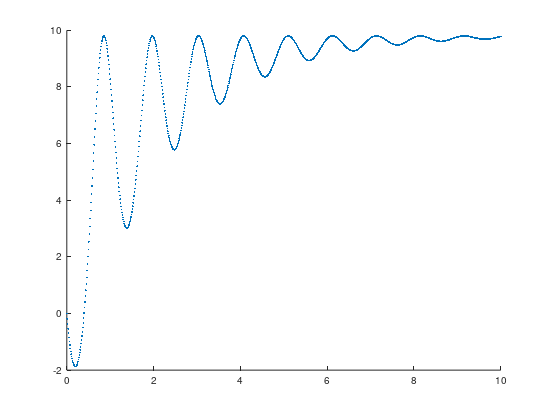
\includegraphics[width=16cm]{img/e2.png}
    \end{figure}

    Se puede observar el claro comportamiento oscilatorio. y la tendencia de equilibrio en 9.8, la cual coincide con el peso del objeto.

    \subsection{Problema 3}

    3. Reproduzca la figura 5.b ($u_1(t) = u_2(t) = 0$) de la referencia [1]

    Para recrear este comportamiento se igualaron las constantes que se utilizan en el artículo

    \begin{align*}
        \beta &= 0.2 \\
        \epsilon_e &= 0.3 \\
        \epsilon_q &= 0 \\ 
        \epsilon_j &= 0.1 \\
        \mu &= 0.000034 \\
        \Lambda &= 408.09 \\
        p &= 0 \\
        k_1 &= 0.1\\
        k_2 &= 0.125\\
        d_1 &= 0.0079\\
        d_2 &= 0.0068 \\
        \sigma_1 &= 0.0337 \\
        \sigma_2 &= 0.0386 \\
    \end{align*}

    En Octave:

    \begin{verbatim}
        beta = 0.2;
        epsilon_e = 0.3;
        epsilon_q = 0;
        epsilon_j = 0.1;
        mu = 0.000034;
        lambda = 408.09;
        p = 0;
        k1 = 0.1;
        k2 = 0.125;
        d1 = 0.0079;
        d2 = 0.0068;
        sigma1 = 0.0337;
        sigma2 = 0.0386;
        tf = 360;
        B1 = 1;
        B2 = 1;
        B3 = 1;
        B4 = 1;
        C1 = 300;
        C2 = 600;
    \end{verbatim}

    El conjunto de funciones derivadas que describen el comportamiento es el siguiente

    \begin{align*}
        \dot{S} &= \Lambda - \frac{S\qty(\beta I + \epsilon_E \beta E + \epsilon_Q \beta Q + \epsilon_J \beta J)}{N} - \mu S \\
        \dot{E} &= p - \frac{S\qty(\beta I + \epsilon_E \beta E + \epsilon_Q \beta Q + \epsilon_J \beta J)}{N} - k_1 E \\
        \dot{Q} &= -(k_2 + \mu) Q \\
        \dot{I} &= k_1 E - \qty(d_1 + \sigma_1 + \mu) I \\
        \dot{J} &= k_2 Q - \qty(d_2 + \sigma_2 + \mu) J \\
        \dot{R} &= \sigma_1 I + \sigma_2 J - \mu R
    \end{align*}

    Entonces se pasan estas funciones como un vector en una sola función en Octave:

    \begin{verbatim}
        fr = @(x,y)
        [(lambda-(y(1)*(beta*y(4)+epsilon_e*beta*y(2)+epsilon_q*beta*y(3)
        +epsilon_j*beta*y(5))/(y(1)+y(2)+y(3)+y(4)+y(5)+y(6))) - mu*y(1)),
        (p + (y(1)*(beta*y(4) + epsilon_e*beta*y(2) + epsilon_q*beta*y(3) +
        epsilon_j*beta*y(5))/(y(1)+y(2)+y(3)+y(4)+y(5)+y(6))) - (k1+mu)*y(2)),
        (-(k2+mu)*y(3)),
        (k1*y(2) - (d1 + sigma1 + mu)*y(4)),
        (k2*y(3) - (d2 + sigma2 + mu)*y(5)),
        (sigma1*y(4) + sigma2*y(5) - mu*y(6))];
    \end{verbatim}

    Y se aplicó el método de Runge Kuta considerando las codniciones iniciales

    \begin{verbatim}
        a=-0;
        b=360;
        y0=[12000000,1565,292,695,326,20];
        npts = 1000;
        sol = RK4(fr,a,b,y0,npts);

        graph = zeros(size(sol)(1),1);

        for i=1:size(sol)(1)
        graph(i,1) = sol(i,3)+sol(i,4)+sol(i,5)+sol(i,6);
        endfor

        hold on;
        scatter(sol(:,1),sol(:,3)+sol(:,4)+sol(:,5)+sol(:,6),5,'filled');
    \end{verbatim}

    Notando que solo se grafican los indiduos activos $E, Q, I, J$.
    
    El resultado gráfico de este método es la siguiente gráfica.

    \begin{figure}[ht!]
        \centering
        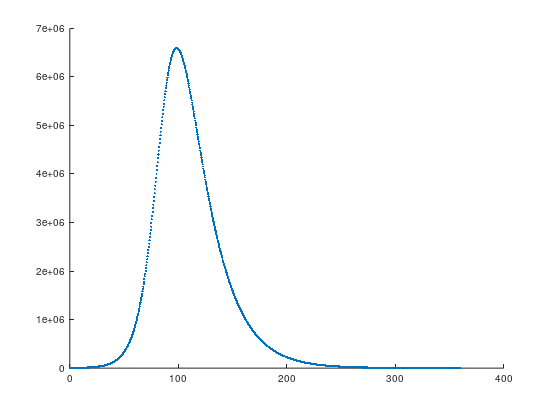
\includegraphics[width=16cm]{img/e3.png}
    \end{figure}

    \subsection{Problema 4}

    4. Implemente los número duales y sobrecargue las siguientes funciones y operadores.

    \verb|(\^), (*), (+), (-), (/), (==), (!=), acos, acosh, asin, asinh, atan,|
    
    \verb|atan2, atanh, sin, cos, cosh, erf, sinh, tan, tanh, exp, log,|
    
    \verb|sqrt, abs|.

    Antes de sobrecargar las funciones se comenzó con una clase que defina las propiedades y métodos de un número dual, se utilizará esta clase para definir los números duales en las operaciones.

    Se creó un directorio llamado \verb|DNFolder/@dual1/| donde se alojará la clase \verb|dual1| en el archivo \verb|dual1.m| con el siguiente código

    \begin{verbatim}
        classdef dual1
            properties
                f0;
                f1;
            endproperties
            methods
                function obj = dual1(g0, g1)
                if(nargin == 1)
                    if(isa(g0,'dual1'))
                        obj = g0;
                        elseif(isnumeric(g0))
                        obj.f0 = g0;
                        obj.f1 = zeros(size(g0));
                    else
                        error('Operation not supported in dual1 constructor')
                    end
                elseif(nargin==2)
                    if(isa(g0, 'dual1') || isa(g1, 'dual1'))
                        error('las componentes del dual1 debe ser reales')
                    elseif(isequal(size(g0), size(g1)))
                        obj.f0 = g0;
                        obj.f1 = g1;
                    endif
                else
                    error('Oparation not supported in dual1 constructor')
                end
                endfunction
            endmethods
        endclassdef
    \end{verbatim}

    Ahora para sobrecargar las funciones se tienen que crear archivos en este mismo directorio con el nombre de la función a sobrecargar y con la función de sobrecarga.

    Por ejemplo para sobrecargar el operador \verb|sum| se crea el archivo \verb|sum.m| con el siguiente código.

    \begin{verbatim}
        function fr = plus(x,y)
            fr = dual1(x.f0 + y.f0, x.f1 + y.f1);
        endfunction
    \end{verbatim}

    Entonces se procede a sobrecargar cada operador y función requerida:

    Operador \verb|power|

    \begin{verbatim}
        function fr = power(x,y)
            r = dual1(x.f0 .^ y.f0, (x.f0 .^ (y.f0-1)) .* 
            (y.f1.*log(x.f0).*x.f0 + y.f0.*x.f1) );
        endfunction
    \end{verbatim}

    Operador \verb|mpower|

    \begin{verbatim}
        function fr = mpower(x,y)
            fr = dual1(x.f0 .^ y.f0, (x.f0 .^ (y.f0-1)) .* 
            (y.f1.*log(x.f0).*x.f0 + y.f0.*x.f1) );
        endfunction
    \end{verbatim}

    Operador \verb|mtimes|

    \begin{verbatim}
        function fr = mtimes(x,y)
            fr = dual1(x.f0 * y.f0, x.f1 * y.f0 + x.f0 * y.f1);
        endfunction
    \end{verbatim}

    Operador \verb|mrdivide|

    \begin{verbatim}
        function fr = mrdivide(x,y)
            fr = dual1(x.f0 / y.f0, (x.f1*y.f0 - x.f0*y.f1)/((y.f0)^2));
        endfunction
    \end{verbatim}

    Operador \verb|rdivide|

    \begin{verbatim}
        function fr = rdivide(x,y)
            fr = dual1(x.f0 / y.f0, (x.f1*y.f0 - x.f0*y.f1)/((y.f0)^2));
        endfunction
    \end{verbatim}
    
    Operador \verb|minus|

    \begin{verbatim}
        function fr = minus(x,y)
            fr = dual1(x.f0 - y.f0, x.f1 - y.f1);
        endfunction
    \end{verbatim}

    Operador lógico \verb|eq|

    \begin{verbatim}
        function fr = eq(x,y)
            fr = dual1(x.f0 == y.f0, x.f1 == y.f1);
        endfunction
    \end{verbatim}

    Operador lógico \verb|ne|

    \begin{verbatim}
        function fr = ne(x,y)
            fr = dual1(x.f0 != y.f0, x.f1 != y.f1);
        endfunction
    \end{verbatim}

    Función \verb|sin|

    \begin{verbatim}
        function fr = sin(g)
            fr = dual1(sin(g.f0), g.f1.*cos(g.f0));
        endfunction
    \end{verbatim}

    Función \verb|cos|

    \begin{verbatim}
        function fr = cos(g)
            fr = dual1(cos(g.f0), -sin(g.f0) .* g.f1);
        endfunction
    \end{verbatim}

    Función \verb|tan|

    \begin{verbatim}
        function fr = tan(x)
            fr = dual1(tan(x.f0), x.f1 ./ ((cos(x.f0))^2));
        endfunction
    \end{verbatim}

    Función \verb|sinh|

    \begin{verbatim}
        function fr = sinh(x)
            fr = dual1(sinh(x.f0), x.f1.*cosh(x.f0));
        endfunction
    \end{verbatim}

    Función \verb|cosh|

    \begin{verbatim}
        function fr = cosh(x)
            fr = dual1(cosh(x.f0), x.f1.*sinh(x.f0));
        endfunction
    \end{verbatim}

    Función \verb|tanh|

    \begin{verbatim}
        function fr = tanh(x)
            fr = dual1(tanh(x.f0), x.f1 ./ ((cosh(x.f0))^2));
        endfunction
    \end{verbatim}

    Función \verb|asin|

    \begin{verbatim}
        function fr = asin(x)
            fr = dual1(asin(x.f0), x.f1 ./ (sqrt(1-(x.f0)^2)));
        endfunction
    \end{verbatim}

    Función \verb|acos|

    \begin{verbatim}
        function fr = acos(x)
            fr = dual1(acos(x.f0), -x.f1 ./ (sqrt(1-(x.f0)^2)));
        endfunction
    \end{verbatim}

    Función \verb|atan|

    \begin{verbatim}
        function fr = atan(x)
            fr = dual1(atan(x.f0), x.f1 ./ (1+(x.f0)^2));
        endfunction
    \end{verbatim}

    Función \verb|asinh|

    \begin{verbatim}
        function fr = asinh(x)
            fr = dual1(asinh(x.f0), x.f1 ./ (sqrt((x.f0)^2+1)));
        endfunction
    \end{verbatim}

    Función \verb|acosh|

    \begin{verbatim}
        function fr = acosh(x)
            fr = dual1(acosh(x.f0), x.f1 ./ (sqrt((x.f0)^2-1)));
        endfunction
    \end{verbatim}

    Función \verb|atanh|

    \begin{verbatim}
        function fr = atanh(x)
            fr = dual1(atanh(x.f0), x.f1 ./ (1-(x.f0)^2));
        endfunction
    \end{verbatim}

    Función \verb|atan2|

    \begin{verbatim}
        function fr = atan2(x,y)
            fr = dual1(atan2(x.f0, y.f0), (y.f0.*x.f1 - x.f0.*y.f1) ./ 
            ((x.f0).^2 + (y.f0).^2));
        endfunction
    \end{verbatim}

    Función \verb|erf|

    \begin{verbatim}
        function fr = erf(x)
            fr = dual1(erf(x.f0), (2/sqrt(pi))*exp(-(x.f0)^2).*x.f1);
        endfunction
    \end{verbatim}

    Función \verb|exp|

    \begin{verbatim}
        function fr = exp(x)
            fr = dual1(exp(x.f0), x.f1.*exp(x.f0));
        endfunction
    \end{verbatim}

    Función \verb|log|

    \begin{verbatim}
        function fr = log(x)
            fr = dual1(log(x.f0), x.f1 ./ x.f0);
        endfunction
    \end{verbatim}

    Función \verb|sqrt|

    \begin{verbatim}
        function fr = sqrt(x)
            fr = dual1(sqrt(x.f0), x.f1 ./ (2*sqrt(x.f0)));
        endfunction
    \end{verbatim}

    Función \verb|abs|

    \begin{verbatim}
        function fr = abs(x)
            fr = dual1(abs(x.f0), (x.f0./abs(x.f0)).*x.f1);
        endfunction
    \end{verbatim}

    Para probar cada una de las funciones se define un número dual de la siguiente forma

    \[
        X_d = 1.1 + \epsilon
    \]

    En Octave llamando la función \verb|dual1|:

    \begin{verbatim}
        xd = dual1(1.1,1);
    \end{verbatim}

    Y se realiza sus operaciones con camptabilidad dual correctamente de la siguiente manera:

    \begin{verbatim}
        xd+xd
        xd-xd
        xd*xd
        xd/xd
        xd^xd
        xd==xd
        xd!=xd
        sin(xd)
        cos(xd)
        tan(xd)
        sinh(xd)
        cosh(xd)
        tanh(xd)
        asin(xd)
        acos(xd)
        atan(xd)
        asinh(xd)
        acosh(xd)
        atanh(xd)
        atan2(xd,xd)
        sqrt(xd)
        exp(xd)
        log(xd)
        erf(xd)
        abs(xd)
    \end{verbatim}

    \subsection{Problema 5}

    5. Usando las funciones del ejercicio anterior, implemente $\nabla f(x0)$ y $Jf(x0)$; una función que permita calcular el gradiente y otra que calcule el Jacobiano de una función evaluada en el punto $x_0$.

    Se propone la función

    \[
        f_t(x,y,z) = \sin(x) + \cos(y)+ \tan(z)
    \]

    en el punto (4,5,6)

    Entonces se definen estos parámetros en Octave:

    \begin{verbatim}
        ft = @(x,y,z) sin(x)+cos(y)+tan(z)
        gt = [4,5,6];
    \end{verbatim}

    Para obtener el gradiente se obtiene la derivada parcial de cada variable de la función propuesta:

    \begin{verbatim}
        a = cell(3,1);

        a(1,1) = ft(dual1(gt(1), 1), dual1(gt(2), 0), dual1(gt(3), 0)).f1;
        a(2,1) = ft(dual1(gt(1), 0), dual1(gt(2), 1), dual1(gt(3), 0)).f1;
        a(3,1) = ft(dual1(gt(1), 0), dual1(gt(2), 0), dual1(gt(3), 1)).f1;
    \end{verbatim}

    El resultado de esta evaluación es que el gradiente de la función en el punto (4,5,6) es

    \[
        \nabla f(4,5,6) = \begin{bmatrix}
            -0.65365 \\
            0.95892 \\
            1.0847
        \end{bmatrix}
    \]

    Por lo tanto la operación funciona.

    El jacobiano es simplemente realizar la misma operación de gradiente en un conjunto de funciones de entrada, con esta operación de obtendrían $n$ derivadas parciales de cada $m$ funciones de entrada, obteniendo una matriz jacobiana de $m \times n$.

    Implementando en Octave un ejemplo con las funciones:

    \begin{align*}
        f_1(x,y,z) &= \sin(x) + \cos(y)+ \tan(z) \\
        f_2(x,y,z) &= \sin(y) + \cos(z)+ \tan(x) \\
        f_3(x,y,z) &= \sin(y) + \cos(x)+ \tan(y) \\
    \end{align*}

    En los puntos (1,2,3), (4,5,6) y (7,8,9)

    \begin{verbatim}
        fj1 = @(x,y,z) sin(x)+cos(y)+tan(z)
        fj2 = @(x,y,z) sin(y)+cos(z)+tan(x)
        fj3 = @(x,y,z) sin(z)+cos(x)+tan(y)

        gj1 = [1,2,3]
        gj2 = [4,5,6]
        gj3 = [7,8,9]
    \end{verbatim}

    Aplicando las operaciones para obtener el jacobiano

    \begin{verbatim}
        b = cell(3,3)

        b(1,1) = fj1(dual1(gj1(1), 1), dual1(gj1(2), 0), dual1(gj1(3), 0)).f1;
        b(2,1) = fj1(dual1(gj1(1), 0), dual1(gj1(2), 1), dual1(gj1(3), 0)).f1;
        b(3,1) = fj1(dual1(gj1(1), 0), dual1(gj1(2), 0), dual1(gj1(3), 1)).f1;

        b(1,2) = fj2(dual1(gj2(1), 1), dual1(gj2(2), 0), dual1(gj2(3), 0)).f1;
        b(2,2) = fj2(dual1(gj2(1), 0), dual1(gj2(2), 1), dual1(gj2(3), 0)).f1;
        b(3,2) = fj2(dual1(gj2(1), 0), dual1(gj2(2), 0), dual1(gj2(3), 1)).f1;

        b(1,3) = fj3(dual1(gj3(1), 1), dual1(gj3(2), 0), dual1(gj3(3), 0)).f1;
        b(2,3) = fj3(dual1(gj3(1), 0), dual1(gj3(2), 1), dual1(gj3(3), 0)).f1;
        b(3,3) = fj3(dual1(gj3(1), 0), dual1(gj3(2), 0), dual1(gj3(3), 1)).f1;
    \end{verbatim}

    El resultado es la matriz jacobiana con el siguiente valor

    \[
        J = \begin{bmatrix}
            0.54030 & -0.90930 & 1.0203 \\
            2.3406 & 0.28366 & 0.27942 \\
            -0.65699 & 47.236 & -0.91113
        \end{bmatrix}
    \]


    


\end{document}